\documentclass[conference]{IEEEtran}
\usepackage{graphicx}
\usepackage{booktabs}
\usepackage{amsmath}
\usepackage{amssymb}
\usepackage{cite}
\usepackage{placeins}
\usepackage{caption}
\usepackage{subcaption}
\usepackage{multirow}
\usepackage{tabularx}
\usepackage{dblfloatfix}
\usepackage{etoolbox}
\usepackage{float}
\usepackage[hidelinks]{hyperref}

\makeatletter
\patchcmd{\thebibliography}{\section*{\refname}}{\section*{\centering\refname}}{}{}
\makeatother

\graphicspath{{figures/}}

\setlength{\textfloatsep}{6pt plus 2pt minus 2pt}
\setlength{\floatsep}{4pt plus 2pt minus 2pt}
\setlength{\intextsep}{6pt plus 2pt minus 2pt}
\captionsetup{font=small,labelfont=bf,skip=3pt}
\captionsetup[subfigure]{font=scriptsize,skip=2pt}

\newcommand{\ie}{\textit{i.e.}}
\newcommand{\eg}{\textit{e.g.}}

\title{Fixed Geometry, Not Learned Residuals:\\
Exposing Ego-Motion Shortcuts in Sensor-Free Pedestrian Trajectory and Intent Prediction}

\author{\IEEEauthorblockN{Anonymous Authors}
\IEEEauthorblockA{Paper under blind review; remove author block for camera-ready}}

\begin{document}
\maketitle

% ======================================================================
\begin{abstract}
Egocentric pedestrian tracks confound pedestrian motion with camera motion.
Zhang~\textit{et al.}~\cite{zhang2024decouple} decompose the mixture using ego-speed as input and soft supervision; LIM~\cite{lim2025tits} deletes speed to avoid causal confusion.
We ask whether classical offline geometry can recover camera motion without any speed sensor, and whether a learned module can reproduce that geometry from tracks alone.
We introduce a standing-pedestrian \emph{variance gate}: for stationary pedestrians while the vehicle moves, valid compensation must satisfy $\mathrm{Var}(\text{comp}) < \mathrm{Var}(\text{raw})$ over the observation window.
Three learned multi-agent residual (LEMC) variants all fail this gate, while full-affine ORB compensation evaluated at each agent's image position passes (93.1\% on PIE, 96.9\% on JAAD).
Fixed ORB is trajectory-neutral on PIE (ADE 60.5 vs.\ 60.8\,px, $-$0.5\%) yet trajectory-improving on JAAD (62.7 vs.\ 83.1\,px, $-$25\%) where no ego-motion sensor exists.
Intent AUC rises monotonically with ego-motion information (0.80 $<$ 0.89 $<$ 0.93), suggesting a substantial share of reported intent accuracy reflects a camera-motion shortcut rather than genuine pedestrian-intent modelling.
\end{abstract}

\begin{IEEEkeywords}
pedestrian trajectory prediction, pedestrian intent prediction, ego-motion compensation, ORB, RANSAC, affine stabilisation, variance gate, causal shortcuts, JAAD, PIE
\end{IEEEkeywords}

% ======================================================================
\section{Introduction}
\label{sec:intro}

Cameras mounted on moving vehicles record the world from a continuously shifting viewpoint.
Every object's image-plane trajectory is therefore a superposition of pedestrian motion and camera motion: a pedestrian standing perfectly still still drifts across the frame as the vehicle advances.
Models that ignore this confound may fit ego-motion patterns rather than pedestrian behaviour, yielding fragile predictions that degrade under domain shift.

Two recent lines of work address this.
Zhang~\textit{et al.}~\cite{zhang2024decouple} decompose the mixture using ego-speed as a soft supervisory signal.
LIM~\cite{lim2025tits} takes the opposite stance: ego-speed is causally entangled with driver reaction and should be removed entirely to avoid shortcut learning.
Both require ego-vehicle odometry, which is available on PIE~\cite{rasouli2019pie} but absent on JAAD~\cite{kotseruba2017jaad}, the larger and more diverse of the two public benchmarks.

We ask a sharper question: can \emph{sensor-free} visual geometry recover camera motion well enough to improve trajectory prediction on both datasets, and can a learned module match that geometry from pedestrian displacement statistics alone?
We study two candidates:
\begin{enumerate}[leftmargin=1.4em,itemsep=1pt,topsep=2pt]
  \item \textbf{Fixed offline ORB affine.} For each frame pair, ORB~\cite{rublee2011orb} keypoints on the background (pedestrian boxes masked) yield a partial affine $M$ via RANSAC~\cite{fischler1981ransac}.
        Compensation is applied \emph{per agent} at its image-plane centre, not as a global translation, capturing position-dependent rotation and scale effects.
  \item \textbf{Learned multi-agent residual (LEMC).} Per-transition displacement statistics (median, trimmed mean, IQR) across all co-visible agents feed a GRU that outputs a 2-D compensation residual.
        We test three supervision regimes: unsupervised, OBD-magnitude auxiliary loss, and direct ORB-regression.
\end{enumerate}
To adjudicate between them without relying solely on downstream ADE, we introduce the \textbf{standing-pedestrian variance gate} as a model-free physical validity test.

\textbf{Contributions.}
\begin{enumerate}[leftmargin=1.4em,itemsep=1pt,topsep=2pt]
  \item Position-dependent full-affine ORB compensation, with a diagnostic ($n{=}300$) showing why global translation fails ($\sim$21\% vs.\ $\sim$89\% gate pass rate).
  \item A reusable variance gate exposing failure of all three LEMC variants despite superficial OBD correlation ($R^2{=}0.30$).
  \item Fixed ORB trajectory-neutral on PIE ($-$0.5\%) and $-$25\% ADE on JAAD, with zero sensor dependence at inference.
  \item Stratified evidence that GT speed \emph{harms} ADE during acceleration and deceleration, corroborating LIM~\cite{lim2025tits}.
  \item Monotonic intent-AUC ordering (compensated $<$ raw $<$ GT speed) isolating an ego-motion shortcut in intent benchmarks.
\end{enumerate}

% ======================================================================
\section{Related Work}
\label{sec:related}

\textbf{Sensor-dependent decomposition.}
Zhang~\textit{et al.}~\cite{zhang2024decouple} weight trajectory loss by ego-speed, reporting ADE 17.41\,px on PIE with I3D visual features; not comparable to our bbox-only GRU.
Czech~\textit{et al.}~\cite{czech2023behavior} subtract predicted ego-motion from pedestrian trajectories using a spatio-temporal module conditioned on odometry and intended route; this is unavailable on JAAD.
Peng~\textit{et al.}~\cite{peng2026trajmamba} encode ego-motion with a dedicated Mamba module to guide pedestrian decoding, again consuming odometry as input.

\textbf{Sensor deletion.}
LIM~\cite{lim2025tits} argues ego-speed creates a causal shortcut between driver reaction and crossing labels and removes it entirely.
Azarmi~\textit{et al.}~\cite{azarmi2024feature}, using permutation-based feature importance across sixteen PIE subsets, independently confirm that ego-speed bias concentrates in yielding (deceleration) scenarios, corroborating our stratified finding (Section~\ref{sec:strat}).

\textbf{Sensor-free visual geometry.}
Neumann and Vedaldi~\cite{neumann2021pedestrian} disentangle pedestrian and ego-motion with a self-supervised CNN on raw video, avoiding speed sensors but requiring pixels at both training and inference.
Our approach differs: pixels are consumed only in an offline ORB extraction pass; inference uses precomputed affines and bbox coordinates only.

\textbf{Classical geometry in visual odometry.}
ORB-based stabilisation is standard in visual odometry~\cite{rublee2011orb} but has not been benchmarked as a position-dependent compensator for pedestrian trajectory prediction under a physical validity test, the gap this paper addresses.

Table~\ref{tab:compare} positions our approach against the above work on five deployment-relevant dimensions.
We stress that ADE comparisons across different backbones are not meaningful; the table focuses on sensor requirements, physical validity, and JAAD compatibility.

\begin{table*}[!t]
\centering
\caption{Qualitative comparison of ego-motion-aware pedestrian predictors. ADE is not directly comparable across different backbones.}
\label{tab:compare}
\footnotesize
\setlength{\tabcolsep}{4pt}
\begin{tabularx}{\textwidth}{@{}l*{5}{>{\centering\arraybackslash}X}@{}}
\toprule
Method & Ego signal & Pixels at inference & JAAD-native & Physical gate & Traj.\ on JAAD \\
\midrule
Zhang~\textit{et al.}~\cite{zhang2024decouple} & OBD / driver action & Yes (I3D) & Re-encoded labels & No & Not reported \\
LIM~\cite{lim2025tits} & None (deleted) & Yes (skeleton) & Yes & No & Not focus \\
Czech~\textit{et al.}~\cite{czech2023behavior} & Odometry + route & Yes & No & No & Not reported \\
Peng~\textit{et al.}~\cite{peng2026trajmamba} & Ego-motion encoder & Yes & No & No & Not reported \\
Neumann~\textit{et al.}~\cite{neumann2021pedestrian} & Learned from video & Yes & No & No & Not reported \\
Learned LEMC (ours) & Multi-agent stats & No & Yes & \textbf{Fail} ($<$1\%) & Worse than base \\
\textbf{Fixed ORB affine (ours)} & \textbf{None} & \textbf{No} & \textbf{Yes} & \textbf{Pass} (93--97\%) & \textbf{$-$25\% ADE} \\
\bottomrule
\end{tabularx}
\end{table*}

\FloatBarrier

% ======================================================================
\section{Method}
\label{sec:method}

Given observation window $\tau$ and prediction horizon $\eta$, we predict future bbox-centre trajectories and crossing intent from track coordinates only; no raw pixels are used at inference.

\subsection{Fixed ORB-affine compensation}
\label{sec:orb_method}
For each consecutive frame pair $(t, t{+}1)$, we extract ORB keypoints from background regions (pedestrian bounding boxes dilated 10\% and masked out), match them across frames, and fit a partial affine transform $M \in \mathbb{R}^{2\times3}$ via \texttt{estimateAffinePartial2D} under RANSAC~\cite{fischler1981ransac}.
The camera displacement at image position $(c_x, c_y)$ is:
\begin{equation}
  \Delta_t(c_x,c_y) = M_t \begin{bmatrix} c_x \\ c_y \\ 1 \end{bmatrix} - \begin{bmatrix} c_x \\ c_y \end{bmatrix}.
\end{equation}
Compensation is accumulated over the observation window: track coordinates $\mathbf{b}_t$ are shifted by $-\sum_{s\leq t}\Delta_s$ into a stabilised frame; the backbone GRU predicts in that frame; predictions are shifted back by the expected future camera displacement before metric computation.
ORB extraction is a one-time offline process; the resulting affines are stored alongside track data.
Fig.~\ref{fig:arch} illustrates the full pipeline.

\begin{figure}[H]
  \centering
  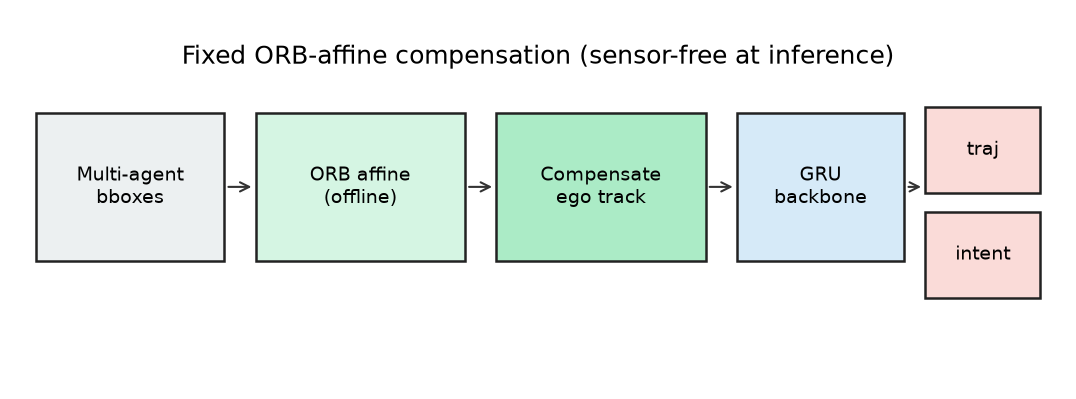
\includegraphics[width=\linewidth,keepaspectratio]{fig2_architecture.png}
  \caption{Fixed ORB-affine pipeline. ORB is extracted offline; at inference only precomputed affines and bbox tracks are required (no pixels, no speed sensor).}
  \label{fig:arch}
\end{figure}

\subsection{Why global translation fails}
\label{sec:translation}
A common simplification keeps only the translation component $(t_x, t_y)$ from $M$, discarding rotation and scale.
Because perspective projection couples rotation and focal length to apparent position-dependent motion, this approximation breaks down for non-central image positions.
On a $n{=}300$ diagnostic set of standing+moving windows, translation-only ORB passes the variance gate on only $\sim$21\% of windows, vs.\ $\sim$89\% for the full affine evaluated per agent.

\subsection{Learned LEMC (ablation)}
\label{sec:lemc_method}
LEMC computes per-transition displacement statistics (median, trimmed mean, IQR) across all co-visible pedestrians and feeds a 2-layer GRU that outputs a 2-D residual, accumulated and subtracted from the ego-pedestrian track.
We ablate three training objectives:
\begin{itemize}[leftmargin=1.2em,itemsep=1pt,topsep=2pt]
  \item \textbf{Unsupervised (no aux.)}: trajectory reconstruction loss only.
  \item \textbf{OBD auxiliary}: additional $\ell_2$ loss on OBD-speed magnitude.
  \item \textbf{ORB-regression}: direct supervision to predict the ORB translation vector.
\end{itemize}

\subsection{Standing-pedestrian variance gate}
\label{sec:gate_method}
For any pedestrian that is stationary (\ie, displacement below a velocity threshold) while the vehicle is moving, a physically valid compensator must reduce track variance:
\begin{equation}
  \mathrm{Var}\!\left(\hat{\mathbf{b}}^{\text{comp}}\right) < \mathrm{Var}\!\left(\hat{\mathbf{b}}^{\text{raw}}\right), \quad \text{over the observation window}.
\end{equation}
We report the fraction of windows satisfying this gate (i) overall and (ii) on the standing+moving subset where the gate is most discriminative.

\FloatBarrier

% ======================================================================
\section{Datasets and Experimental Setup}
\label{sec:setup}

\textbf{PIE}~\cite{rasouli2019pie} was recorded in six urban areas with a dashboard camera at 30\,fps.
After applying Zhang~\textit{et al.}'s~\cite{zhang2024decouple} protocol ($\tau{=}16$ frames observed, $\eta{=}45$ frames predicted, TTE $\in[30,60]$, 50\% sliding-window overlap), we obtain 1,773 test windows.
We densify the multi-agent track store via detection interpolation, yielding a median of 8 co-visible agents per frame.
PIE provides per-frame OBD speed, enabling the GT-speed oracle condition.
Fig.~\ref{fig:datasets} (left) shows the PIE agent density after augmentation.

\textbf{JAAD}~\cite{kotseruba2017jaad,kotseruba2021benchmark} covers 346 video clips from North America and Europe with diverse weather and lighting.
No continuous odometry is available, making it the critical test for sensor-free claims.
ORB affines are extracted from 124 clips with associated video; 295 test windows are used for evaluation.
Fig.~\ref{fig:datasets} (right) shows the JAAD agent density.

\begin{figure}[H]
  \centering
  \begin{subfigure}[t]{0.48\linewidth}
    \centering
    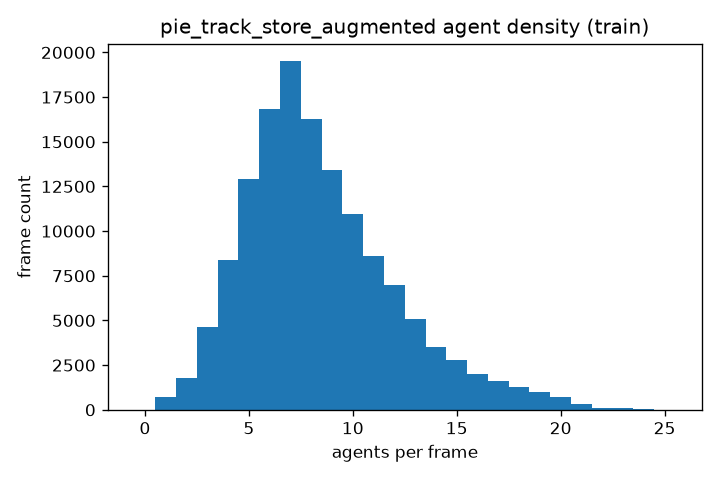
\includegraphics[width=\linewidth,height=0.13\textheight,keepaspectratio]{density_pie_track_store_augmented_train.png}
    \caption{PIE augmented (train)}
  \end{subfigure}\hfill
  \begin{subfigure}[t]{0.48\linewidth}
    \centering
    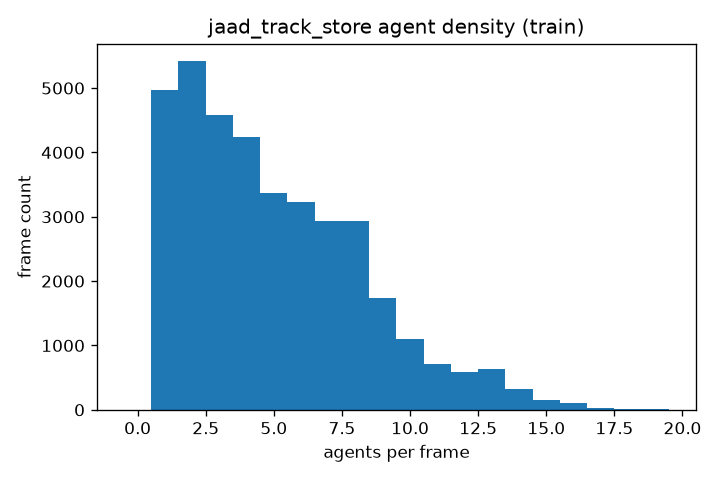
\includegraphics[width=\linewidth,height=0.13\textheight,keepaspectratio]{density_jaad_track_store_train.png}
    \caption{JAAD (train)}
  \end{subfigure}
  \caption{Agent track density per frame. Denser PIE (augmented) provides richer multi-agent context for LEMC; JAAD has sparser tracks on average.}
  \label{fig:datasets}
\end{figure}

\textbf{Backbone.}
A lightweight linear embedding followed by a 2-layer GRU predicts future bbox-centre trajectories and a binary crossing-intent logit.
The backbone is deliberately simple: capacity improvements would mask compensation effects.
All models share the same backbone; the only variation is the compensation applied to input tracks.

\textbf{Metrics.}
\begin{itemize}[leftmargin=1.2em,itemsep=1pt,topsep=2pt]
  \item \textbf{ADE/FDE}: average/final displacement error on bbox centres (pixels).
  \item \textbf{ARB/FRB@30f}: average/final relative displacement error at 30 frames, following Zhang~\textit{et al.}~\cite{zhang2024decouple}.
  \item \textbf{AUC/F1}: intent prediction area under ROC and macro F1.
  \item \textbf{Gate pass rate}: fraction of standing+moving windows satisfying $\mathrm{Var}(\text{comp})<\mathrm{Var}(\text{raw})$.
\end{itemize}
All results are mean $\pm$ std over 3 independent random seeds.
ORB extraction and detection densification are entirely offline; at inference only precomputed affines and bbox coordinates are required.

\FloatBarrier
\newpage

% ======================================================================
\section{Results}
\label{sec:results}

We structure the evaluation in four stages.
First (\S\ref{sec:res_pie}) we compare all methods on downstream PIE trajectory and intent metrics.
Second (\S\ref{sec:res_gate}) we apply the variance gate to ask whether compensation is physically valid \emph{before} interpreting those metrics.
Third (\S\ref{sec:strat}) we stratify PIE ADE by ego-vehicle state and validate ORB against OBD speed.
Fourth (\S\ref{sec:res_jaad}) we evaluate on JAAD and analyse the intent shortcut.

% ---- PIE main grid ----
\subsection{PIE: main comparison}
\label{sec:res_pie}

Table~\ref{tab:pie} reports trajectory and intent metrics for all conditions.
Fixed ORB matches baseline ADE (60.5 vs.\ 60.8\,px) and improves ARB (32.3 vs.\ 34.0\,px) and FRB (54.5 vs.\ 56.5\,px).
All three LEMC variants substantially degrade trajectory quality (ADE $\geq$81.7\,px), including the variant supervised to directly regress ORB translation.
GT-speed conditioning raises intent AUC to 0.93 and F1 to 0.85 but hurts trajectory ADE (67.0\,px) and ARB (36.2\,px), consistent with causal entanglement~\cite{lim2025tits}.
Fig.~\ref{fig:grid} visualises the ADE ordering across all conditions and seeds; the pattern is consistent.

\begin{table*}[!t]
\centering
\caption{PIE test set, mean$\pm$std over 3 seeds. Bold: best trajectory metric. Italic: best intent metric.}
\label{tab:pie}
\footnotesize
\setlength{\tabcolsep}{4pt}
\begin{tabular}{@{}lcccccc@{}}
\toprule
Method & ADE (px) & FDE (px) & ARB (px) & FRB (px) & AUC & F1 \\
\midrule
Baseline (no compensation) & 60.8$\pm$3.3 & 121.8$\pm$9.9 & 34.0$\pm$1.4 & 56.5$\pm$4.3 & 0.89$\pm$0.01 & 0.74$\pm$0.03 \\
GT OBD speed (oracle) & 67.0$\pm$1.3 & 136.9$\pm$3.0 & 36.2$\pm$1.8 & 59.7$\pm$2.1 & \textit{0.93$\pm$0.01} & \textit{0.85$\pm$0.02} \\
\midrule
LEMC, no auxiliary & 81.7$\pm$5.1 & 159.9$\pm$2.4 & 44.2$\pm$4.4 & 70.6$\pm$3.2 & 0.77$\pm$0.05 & 0.64$\pm$0.01 \\
LEMC + OBD auxiliary & 85.8$\pm$11.2 & 164.3$\pm$11.3 & 47.4$\pm$8.2 & 73.6$\pm$6.7 & 0.80$\pm$0.01 & 0.60$\pm$0.03 \\
LEMC + ORB-regression & 81.7$\pm$4.6 & 163.5$\pm$7.6 & 43.7$\pm$2.3 & 71.9$\pm$5.5 & 0.81$\pm$0.01 & 0.63$\pm$0.00 \\
\midrule
\textbf{Fixed ORB affine (ours)} & \textbf{60.5$\pm$1.8} & 130.3$\pm$1.3 & \textbf{32.3$\pm$1.8} & \textbf{54.5$\pm$0.4} & 0.80$\pm$0.01 & 0.60$\pm$0.01 \\
\bottomrule
\end{tabular}
\end{table*}

\begin{figure}[H]
  \centering
  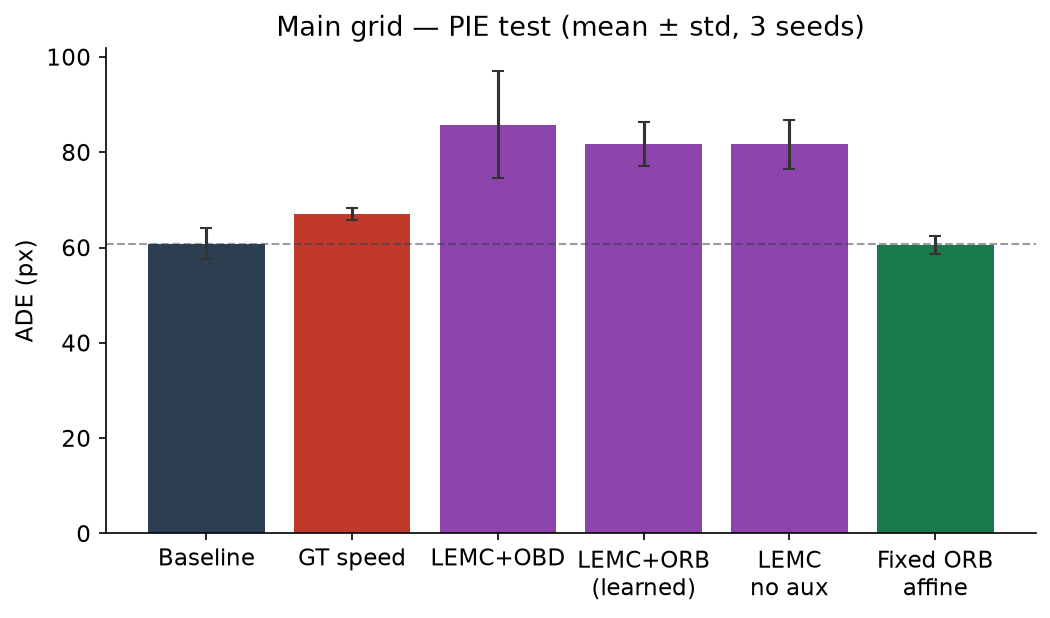
\includegraphics[width=\linewidth,height=0.20\textheight,keepaspectratio]{fig_main_grid_ade.png}
  \caption{PIE ADE across all conditions (3 seeds). Fixed ORB matches the uncompensated baseline; all LEMC variants are substantially worse.}
  \label{fig:grid}
\end{figure}

\FloatBarrier
\newpage

% ---- Physical validity ----
\subsection{Physical validity: variance gate}
\label{sec:res_gate}

Table~\ref{tab:gate} reports gate pass rates.
The key finding is that OBD-supervised LEMC, despite exhibiting $R^2{=}0.30$ correlation with OBD speed (Fig.~\ref{fig:gatediag}b), passes the standing-pedestrian gate on only 0.8\% of standing+moving windows.
Translation-only ORB fares better but still fails 79\% of windows.
Full affine ORB, evaluated per agent, passes 93.1\% on PIE and 96.9\% on JAAD.

This ordering holds at both diagnostic scale ($n{=}300$) and full test scale, demonstrating that the gate generalises.
The failure of LEMC is not due to insufficient data or capacity: the ORB-regression variant, trained to directly predict ORB translations, also fails (33.4\%).
The root cause is that multi-agent statistics cannot distinguish pedestrian motion from coherent camera motion when the two are confounded by position-dependent perspective effects.

\begin{table}[H]
\centering
\caption{Variance gate: fraction of windows satisfying $\mathrm{Var}(\text{comp})<\mathrm{Var}(\text{raw})$ on standing pedestrians.}
\label{tab:gate}
\footnotesize
\setlength{\tabcolsep}{3pt}
\begin{tabular}{@{}llcc@{}}
\toprule
Method & Dataset / scope & All (\%) & Stand.+mov.\ (\%) \\
\midrule
ORB translation only & PIE diag.\ ($n{=}300$) & \multicolumn{2}{c}{$\sim$21} \\
Fixed affine (per-agent) & PIE diag.\ ($n{=}300$) & \multicolumn{2}{c}{$\sim$89} \\
\midrule
LEMC + OBD aux. & PIE test & 0.7 & 0.8 \\
LEMC + ORB-reg. & PIE test & -- & 33.4 \\
\textbf{Fixed ORB} & \textbf{PIE test} & \textbf{76.7} & \textbf{93.1} \\
\textbf{Fixed ORB} & \textbf{JAAD test} & \textbf{71.9} & \textbf{96.9} \\
\bottomrule
\end{tabular}
\end{table}

\begin{figure}[H]
  \centering
  \begin{subfigure}[t]{0.48\linewidth}
    \centering
    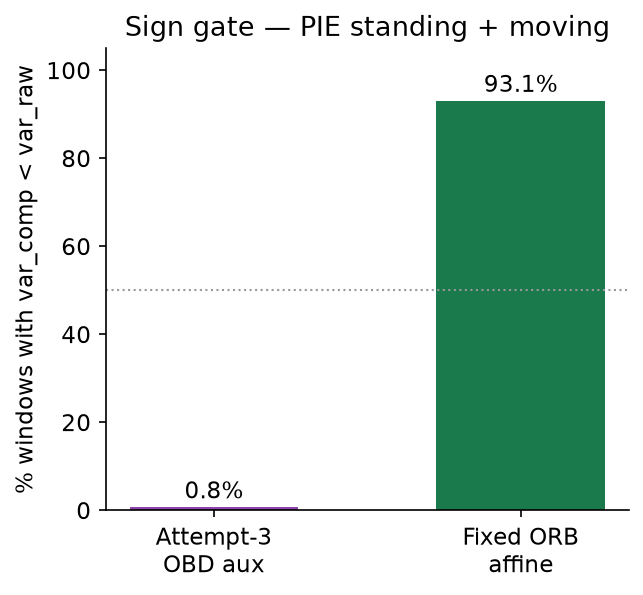
\includegraphics[width=\linewidth,height=0.16\textheight,keepaspectratio]{pie_sign_gate.png}
    \caption{PIE sign gate}
  \end{subfigure}\hfill
  \begin{subfigure}[t]{0.48\linewidth}
    \centering
    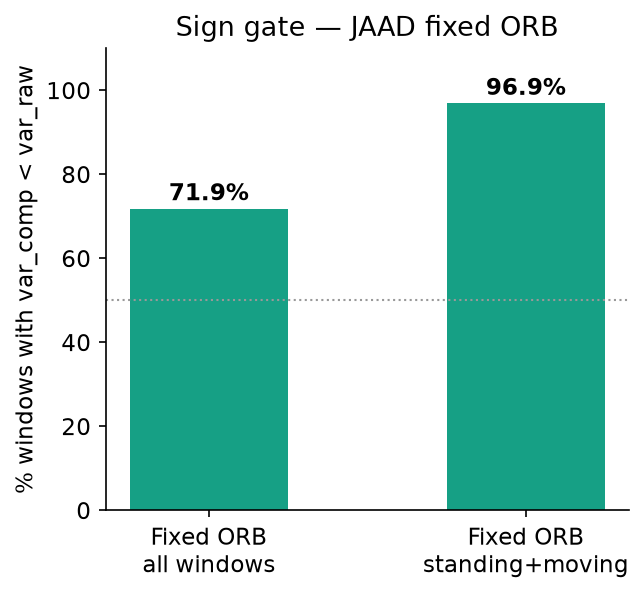
\includegraphics[width=\linewidth,height=0.16\textheight,keepaspectratio]{jaad_sign_gate.png}
    \caption{JAAD sign gate}
  \end{subfigure}\\[4pt]
  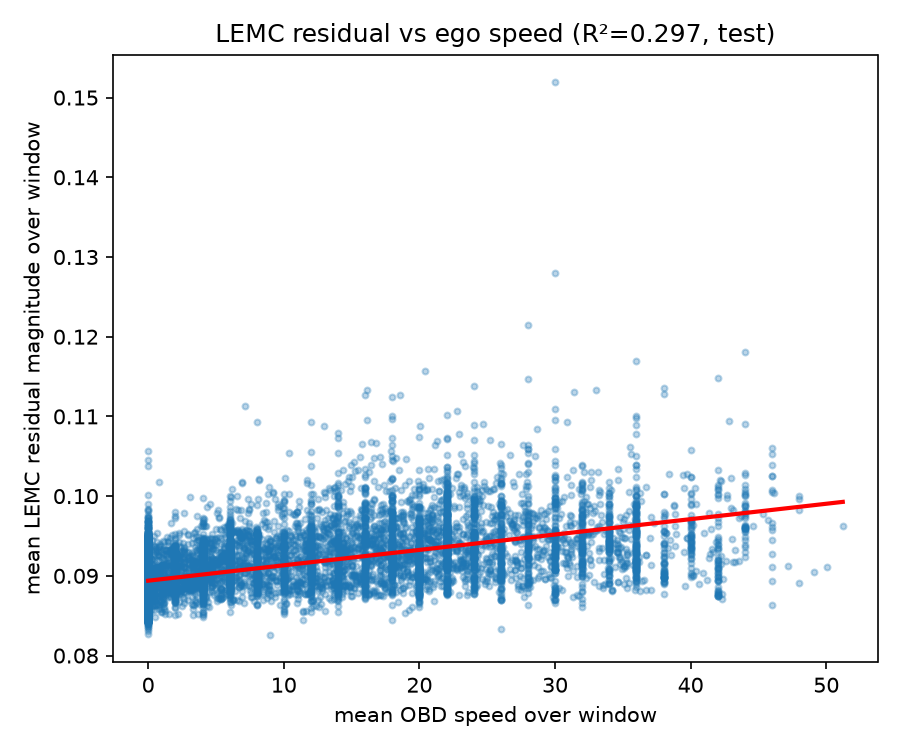
\includegraphics[width=\linewidth,height=0.14\textheight,keepaspectratio]{lemc_obd_scatter_pie_lemc_augmented_auxobd_seed0_test.png}
  \caption*{\scriptsize (c) LEMC residual vs.\ OBD speed ($R^2{=}0.30$): correlated but physically invalid.}
  \caption{Variance gate results on PIE (a) and JAAD (b); OBD correlation of LEMC (c). Fixed ORB passes on both datasets.}
  \label{fig:gatediag}
\end{figure}

\FloatBarrier
\newpage

% ---- ORB validation + stratified ----
\subsection{ORB geometry validation and stratified PIE}
\label{sec:strat}

Fig.~\ref{fig:stratdiag}a plots ORB translation magnitude against simultaneously recorded OBD speed over $n{=}75{,}268$ frame pairs, yielding $R^2{=}0.41$.
This confirms that ORB tracks genuine camera motion without consuming ego-vehicle state at inference: the correlation arises from shared physical dynamics, not from data leakage.

Table~\ref{tab:strat} stratifies ADE/FDE by ego-vehicle acceleration state.
Under acceleration, GT-speed conditioning yields the worst ADE (88.6\,px vs.\ baseline 58.5\,px), while fixed ORB achieves the best (52.2\,px).
The pattern reverses slightly under constant speed, where GT speed is marginally beneficial.
Under deceleration, GT speed again degrades ADE (82.0 vs.\ 65.0\,px baseline).
This exactly reproduces LIM's~\cite{lim2025tits} causal-confusion finding on an independent GRU-only backbone, providing corroborating evidence from a different architectural family.
Fig.~\ref{fig:stratdiag}b visualises the stratified ADE breakdown.

\begin{table}[H]
\centering
\caption{ADE / FDE (px) by ego-vehicle state, PIE seed 0. Bold: best per state.}
\label{tab:strat}
\footnotesize
\setlength{\tabcolsep}{3pt}
\begin{tabular}{@{}lccc@{}}
\toprule
Ego state ($n$) & Baseline & GT speed & Fixed ORB \\
\midrule
Accelerating (251) & 58.5 / 127.8 & 88.6 / 173.2 & \textbf{52.2} / \textbf{122.6} \\
Constant (1364)    & 64.5 / 130.6 & \textbf{62.2} / \textbf{120.3} & 59.4 / 130.1 \\
Decelerating (158) & 65.0 / 139.8 & 82.0 / 174.7 & \textbf{67.5} / \textbf{151.5} \\
\bottomrule
\end{tabular}
\end{table}

\begin{figure}[H]
  \centering
  \begin{subfigure}[t]{0.48\linewidth}
    \centering
    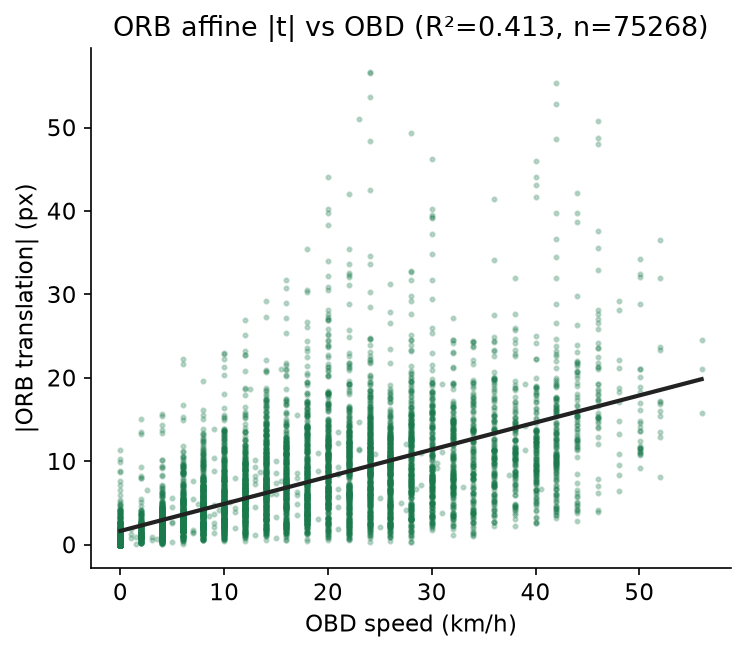
\includegraphics[width=\linewidth,height=0.15\textheight,keepaspectratio]{fig4_orb_obd_scatter.png}
    \caption{ORB $|t|$ vs.\ OBD ($R^2{=}0.41$)}
  \end{subfigure}\hfill
  \begin{subfigure}[t]{0.48\linewidth}
    \centering
    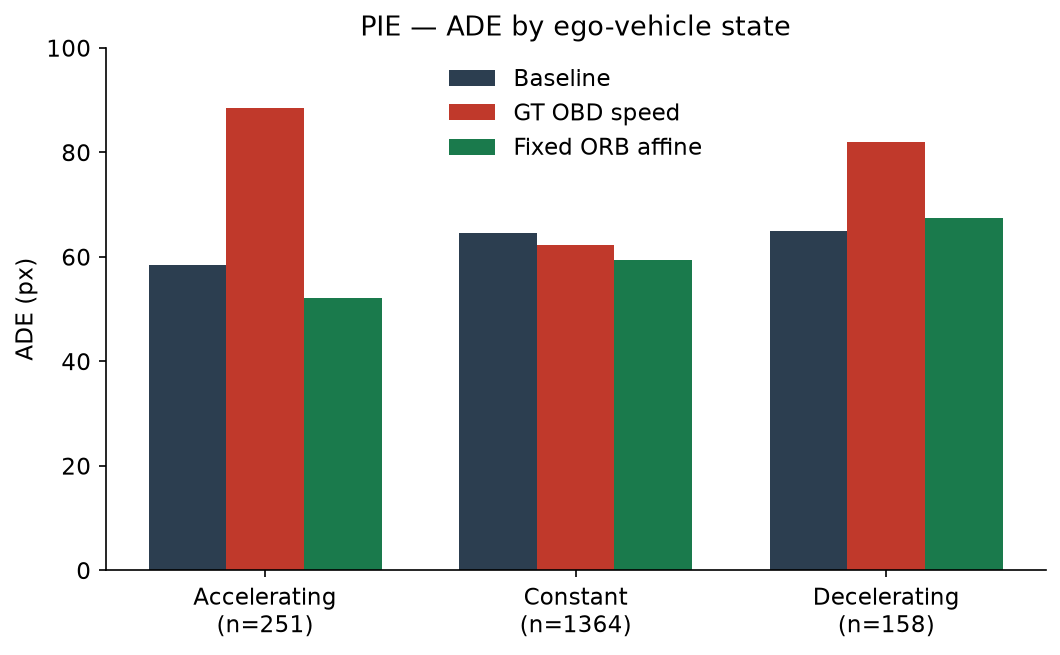
\includegraphics[width=\linewidth,height=0.15\textheight,keepaspectratio]{pie_stratified_ade.png}
    \caption{Stratified ADE by ego state}
  \end{subfigure}
  \caption{ORB geometry validation (a) and stratified PIE ADE (b). GT-speed conditioning degrades trajectory accuracy during ego-acceleration and deceleration.}
  \label{fig:stratdiag}
\end{figure}

\FloatBarrier
\newpage

% ---- JAAD ----
\subsection{JAAD: cross-dataset generalisation}
\label{sec:res_jaad}

JAAD~\cite{kotseruba2017jaad} provides no continuous ego-motion signal; all models operate purely from visual tracks and precomputed ORB affines.
Table~\ref{tab:jaad} shows that fixed ORB reduces ADE by 25\% (83.1 $\rightarrow$ 62.7\,px), FDE by 23\%, ARB by 22\%, and FRB by 24\%.
These are among the largest absolute improvements on JAAD reported under a bbox-only GRU baseline.
Intent AUC remains at chance ($\sim$0.44); JAAD gains are entirely in trajectory prediction.

Fig.~\ref{fig:jaadgrid} shows the JAAD metric grid across seeds; Fig.~\ref{fig:jaadtraj} shows representative windows where compensation reduces ADE from 391\,px to 45\,px and from 435\,px to 94\,px respectively.
The training dynamics on JAAD are shown in Fig.~\ref{fig:training}, demonstrating stable convergence for both conditions.

\begin{table*}[!t]
\centering
\caption{JAAD test set ($n{=}295$), mean$\pm$std over 3 seeds. No GT speed is available; both methods use only precomputed affines and bbox tracks.}
\label{tab:jaad}
\footnotesize
\setlength{\tabcolsep}{5pt}
\begin{tabular}{@{}lcccccc@{}}
\toprule
Method & ADE (px) & FDE (px) & ARB (px) & FRB (px) & AUC & F1 \\
\midrule
Baseline (no compensation) & 83.1$\pm$2.0 & 156.3$\pm$4.3 & 44.8$\pm$2.2 & 71.2$\pm$2.1 & 0.47$\pm$0.05 & 0.90$\pm$0.00 \\
\textbf{Fixed ORB affine (ours)} & \textbf{62.7$\pm$2.3} & \textbf{120.1$\pm$2.8} & \textbf{34.8$\pm$2.3} & \textbf{54.2$\pm$0.9} & 0.44$\pm$0.00 & 0.90$\pm$0.00 \\
\midrule
\multicolumn{7}{l}{\footnotesize \textbf{Improvement:} ADE $-$24.5\%, FDE $-$23.2\%, ARB $-$22.3\%, FRB $-$23.9\%. Intent AUC stays at chance on JAAD.} \\
\bottomrule
\end{tabular}
\end{table*}

\begin{figure}[H]
  \centering
  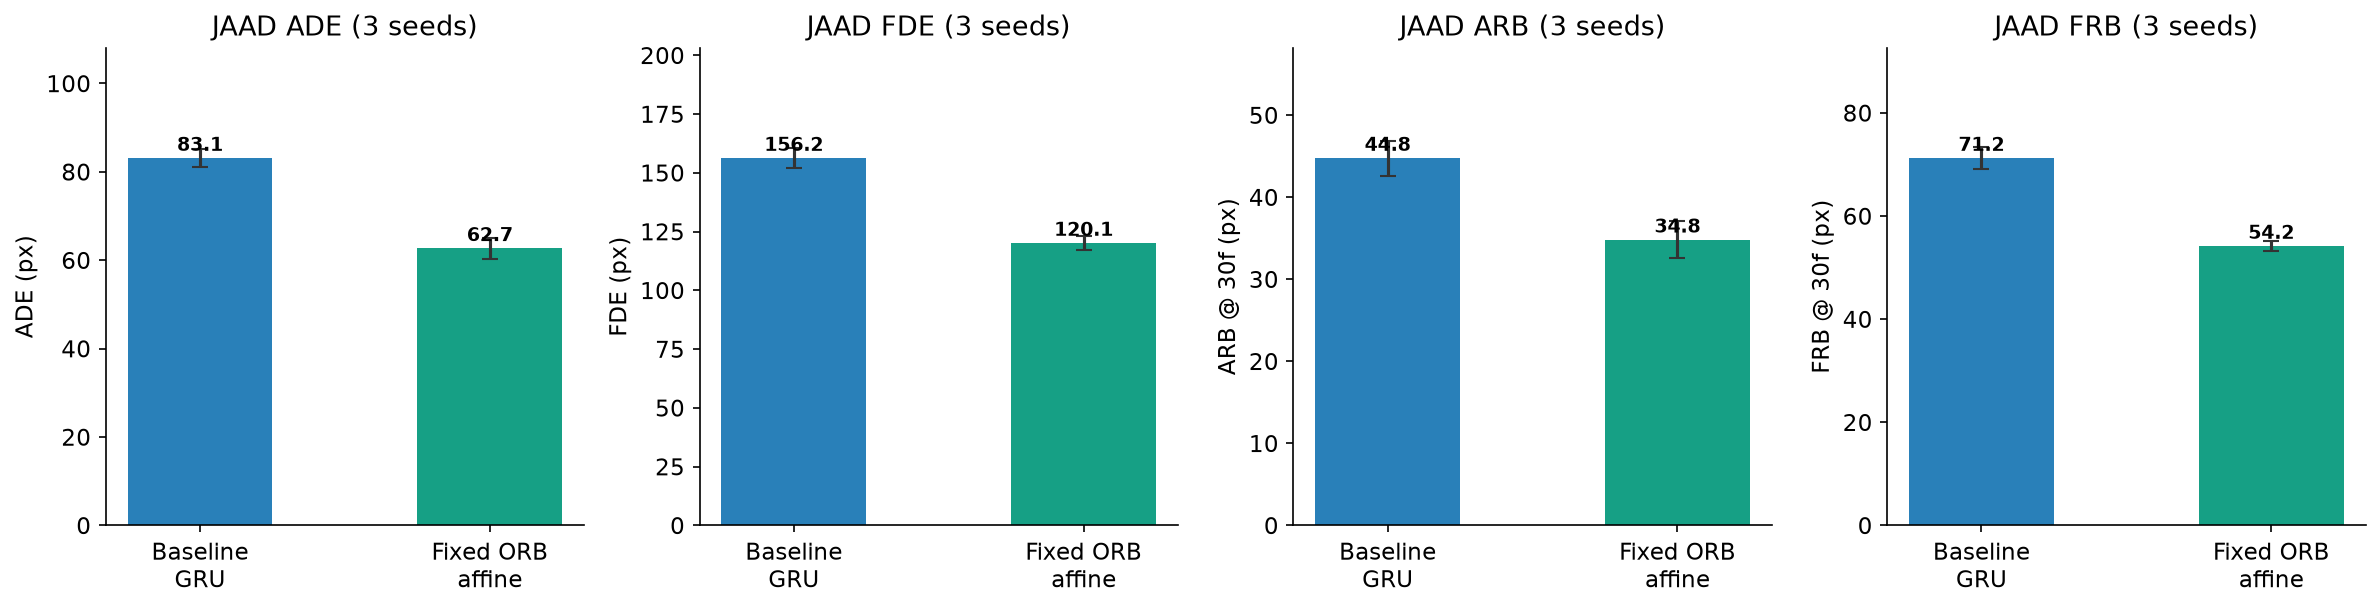
\includegraphics[width=\linewidth,height=0.18\textheight,keepaspectratio]{jaad_grid_metrics.png}
  \caption{JAAD metric grid (3 seeds). Fixed ORB consistently improves all trajectory metrics; intent AUC stays at chance level.}
  \label{fig:jaadgrid}
\end{figure}

\begin{figure}[H]
  \centering
  \begin{subfigure}[t]{0.48\linewidth}
    \centering
    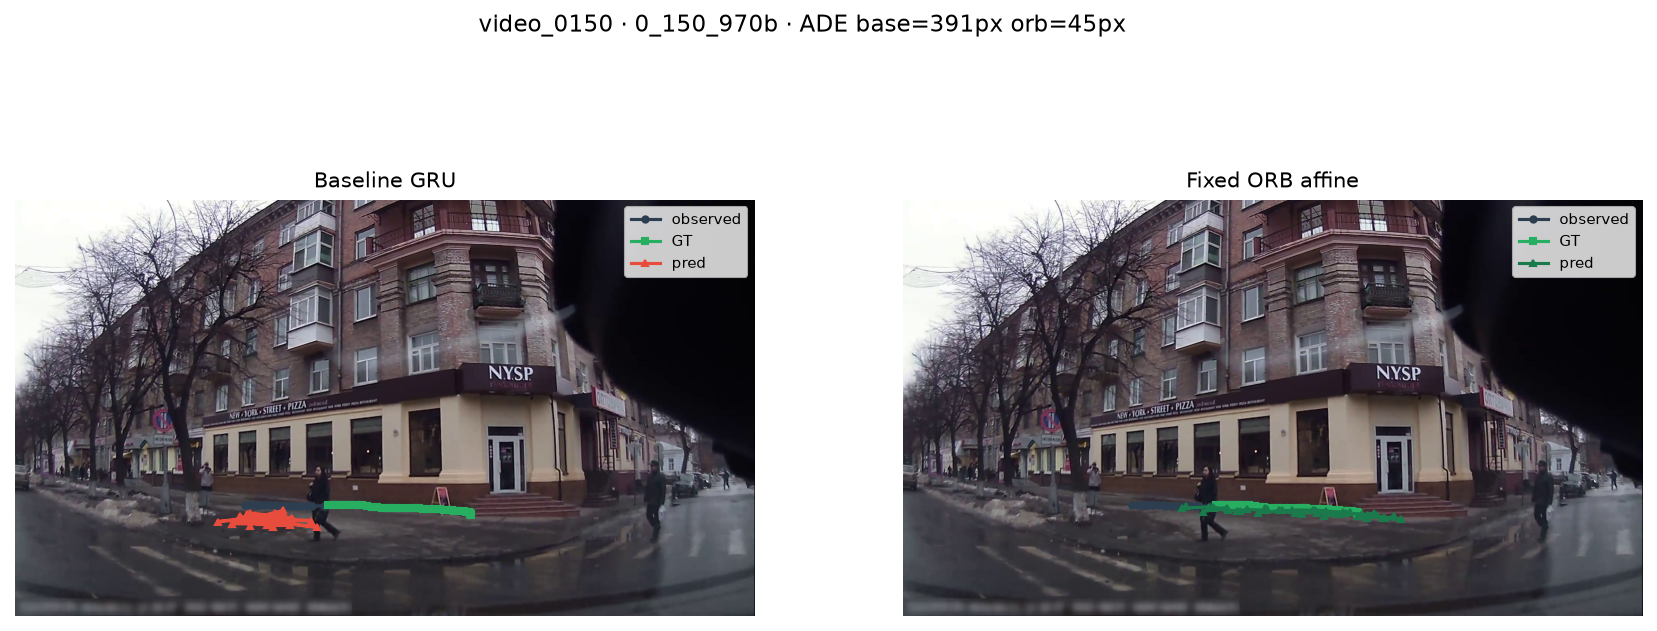
\includegraphics[width=\linewidth,height=0.15\textheight,keepaspectratio]{jaad_compare_0.png}
    \caption{Video 0150: 391$\rightarrow$45\,px}
  \end{subfigure}\hfill
  \begin{subfigure}[t]{0.48\linewidth}
    \centering
    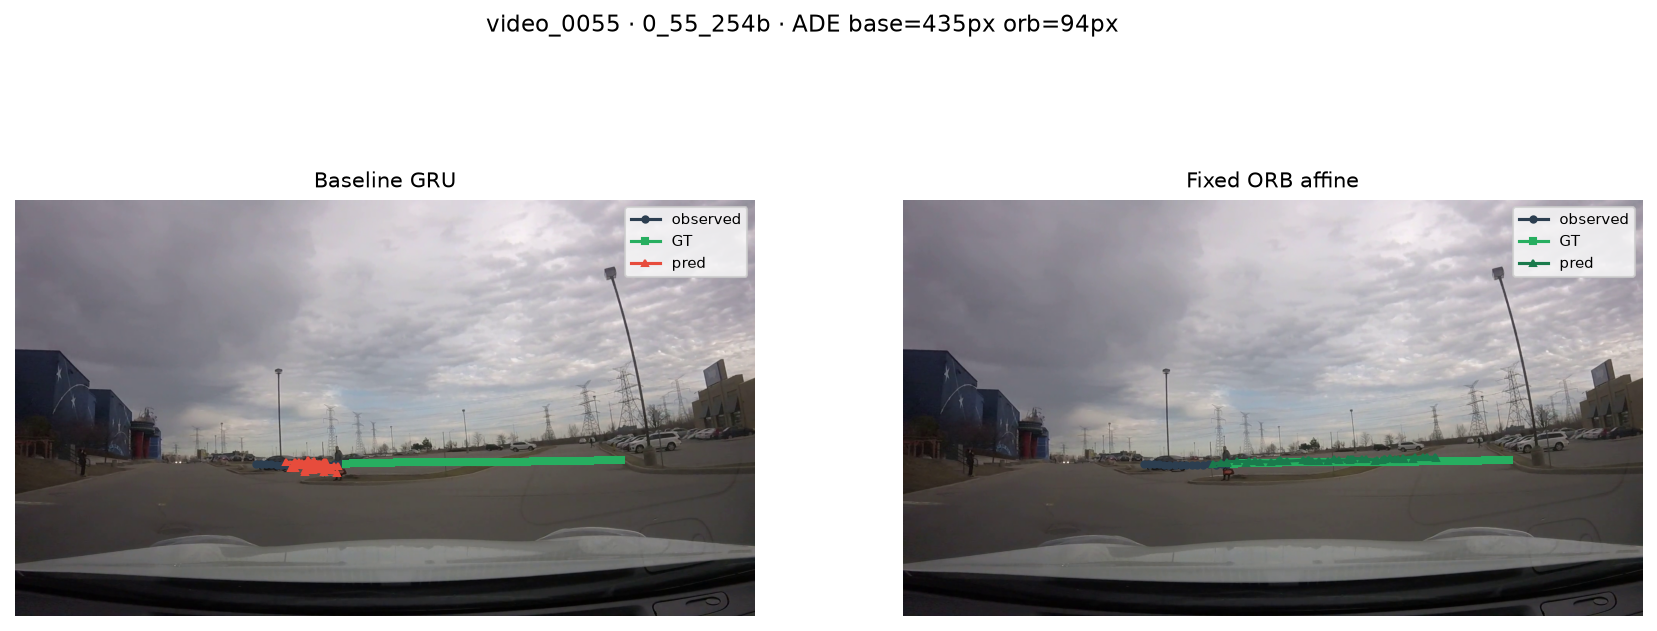
\includegraphics[width=\linewidth,height=0.15\textheight,keepaspectratio]{jaad_compare_1.png}
    \caption{Video 0055: 435$\rightarrow$94\,px}
  \end{subfigure}
  \caption{Representative JAAD trajectory overlays. Blue: baseline; orange: fixed ORB (compensated). Large errors collapse after compensation.}
  \label{fig:jaadtraj}
\end{figure}

\begin{figure}[H]
  \centering
  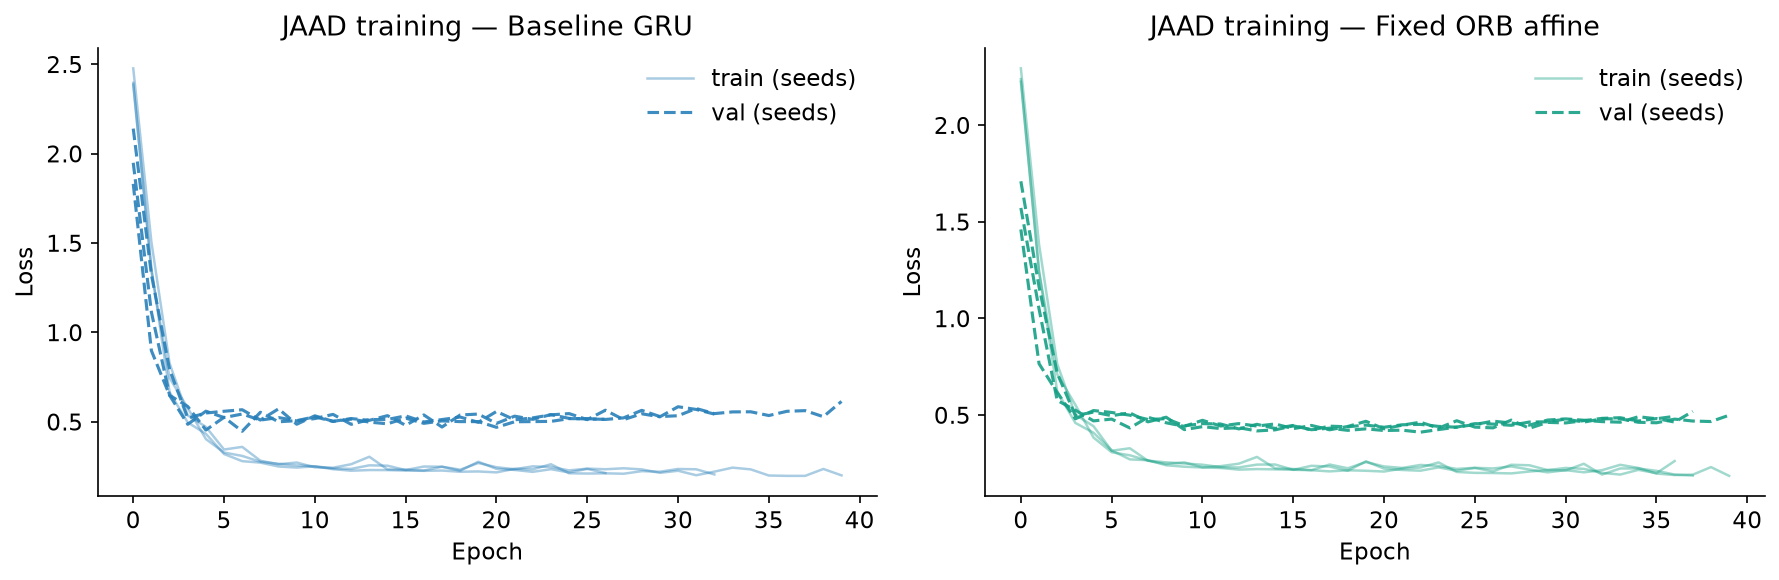
\includegraphics[width=\linewidth,height=0.15\textheight,keepaspectratio]{jaad_training_curves.png}
  \caption{JAAD training curves (seed 0). Both baseline and fixed ORB converge stably; ORB converges to lower validation ADE.}
  \label{fig:training}
\end{figure}

\FloatBarrier
\newpage

% ---- Cross-dataset + intent + qualitative ----
\subsection{Cross-dataset summary and intent shortcut}
\label{sec:res_intent}

Fig.~\ref{fig:cross} compares ADE on PIE and JAAD side-by-side.
Fixed ORB is essentially neutral on PIE ($-$0.5\%) yet substantially better on JAAD ($-$25\%), demonstrating that the gain does not arise from overfitting the compensation to a single dataset but rather from removing genuine ego drift that is more pronounced when no OBD pre-alignment is available.

Intent AUC on PIE rises monotonically with ego-motion exposure: fixed ORB (0.80) $<$ baseline (0.89) $<$ GT speed (0.93); F1 follows the same ordering (0.60 $<$ 0.74 $<$ 0.85).
Fig.~\ref{fig:intent} plots this ordering.
Under LIM's~\cite{lim2025tits} causal account, each step towards more ego-motion information injects spurious cues that inflate apparent intent accuracy: the baseline entangles pedestrian intent with driver braking, GT speed amplifies this, and compensation partially decouples the signal.
This suggests that published PIE intent numbers should be interpreted cautiously unless ego-motion has been explicitly removed.

\begin{figure}[H]
  \centering
  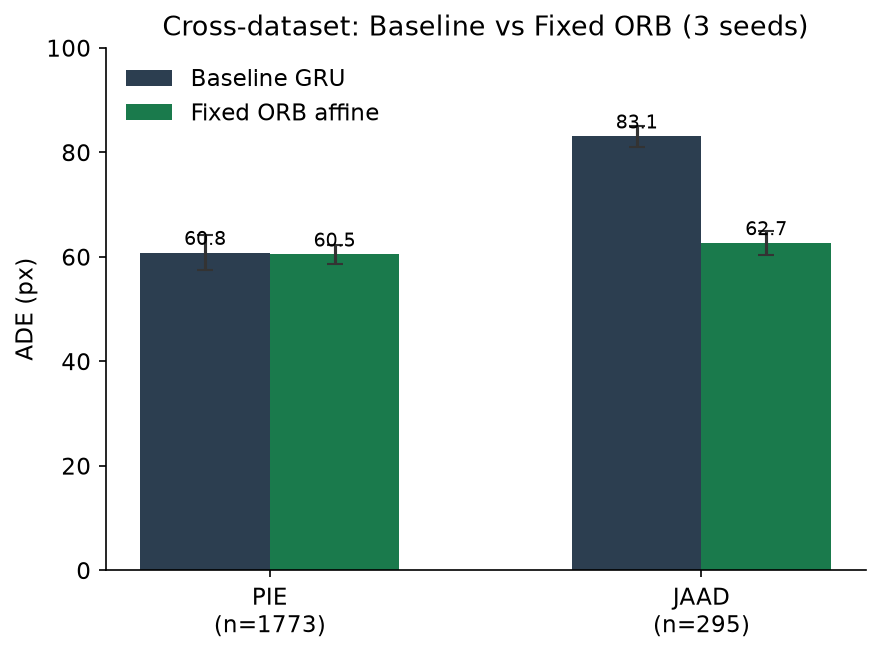
\includegraphics[width=\linewidth,height=0.17\textheight,keepaspectratio]{cross_dataset_ade.png}
  \caption{Cross-dataset ADE comparison. Fixed ORB is neutral on PIE (where raw tracks partially reflect OBD context) and achieves $-$25\% on JAAD (where no ego-motion signal pre-aligns tracks).}
  \label{fig:cross}
\end{figure}

\begin{figure}[H]
  \centering
  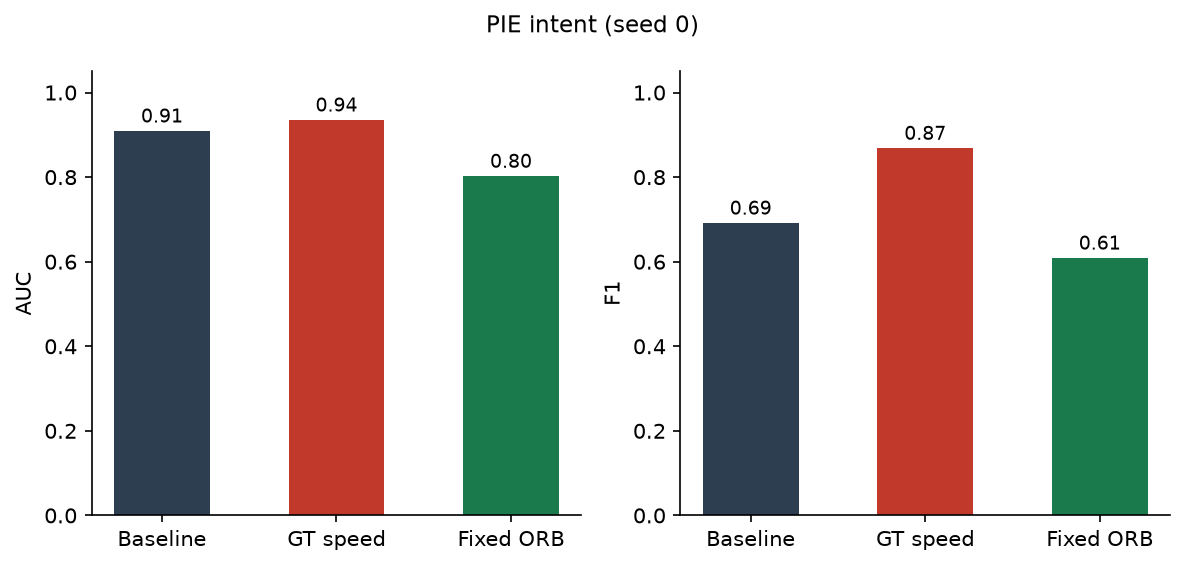
\includegraphics[width=\linewidth,height=0.17\textheight,keepaspectratio]{pie_intent_auc_f1.png}
  \caption{PIE intent AUC and F1 (3-seed means). AUC rises monotonically with ego-motion exposure, consistent with an ego-motion shortcut in intent labels.}
  \label{fig:intent}
\end{figure}

\subsection{Qualitative analysis}
\label{sec:res_qual}

Fig.~\ref{fig:qual} illustrates four complementary views.
Panel (a) shows a standing pedestrian at 18.6\,km/h vehicle speed: the raw track drifts substantially while the compensated track stays near-stationary, confirming the variance gate finding visually.
Panel (b) shows a PIE trajectory overlay on a real frame.
Panel (c) shows the LEMC OBD-scatter for the OBD-auxiliary variant: despite apparent speed correlation, the residuals are physically meaningless.
Panel (d) shows a LEMC failure case: the compensated track loops instead of flattening, confirming that multi-agent statistics fit displacement noise rather than coherent camera motion.

\begin{figure}[H]
  \centering
  \begin{subfigure}[t]{0.48\linewidth}
    \centering
    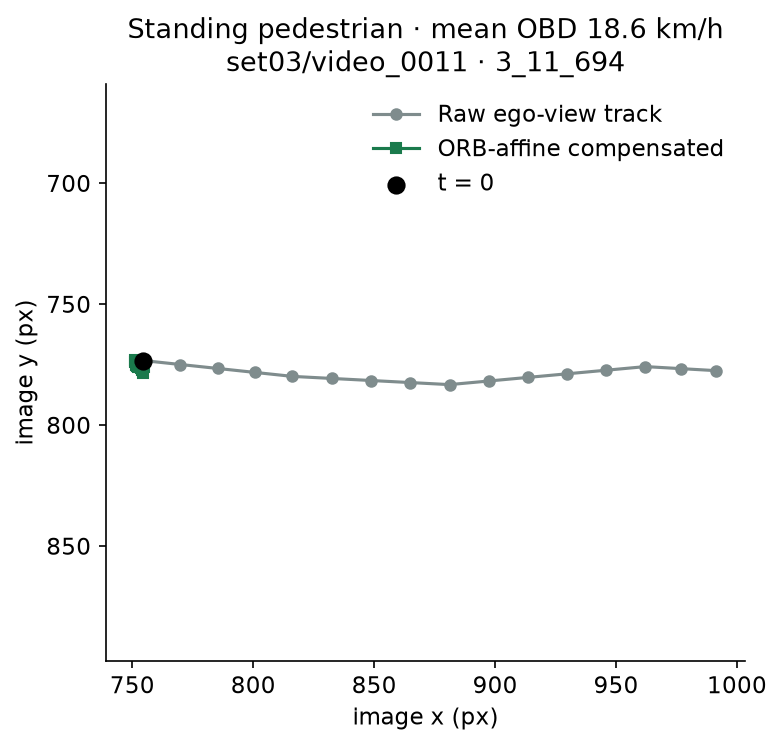
\includegraphics[width=\linewidth,height=0.16\textheight,keepaspectratio]{fig1_teaser.png}
    \caption{Standing pedestrian (18.6\,km/h)}
  \end{subfigure}\hfill
  \begin{subfigure}[t]{0.48\linewidth}
    \centering
    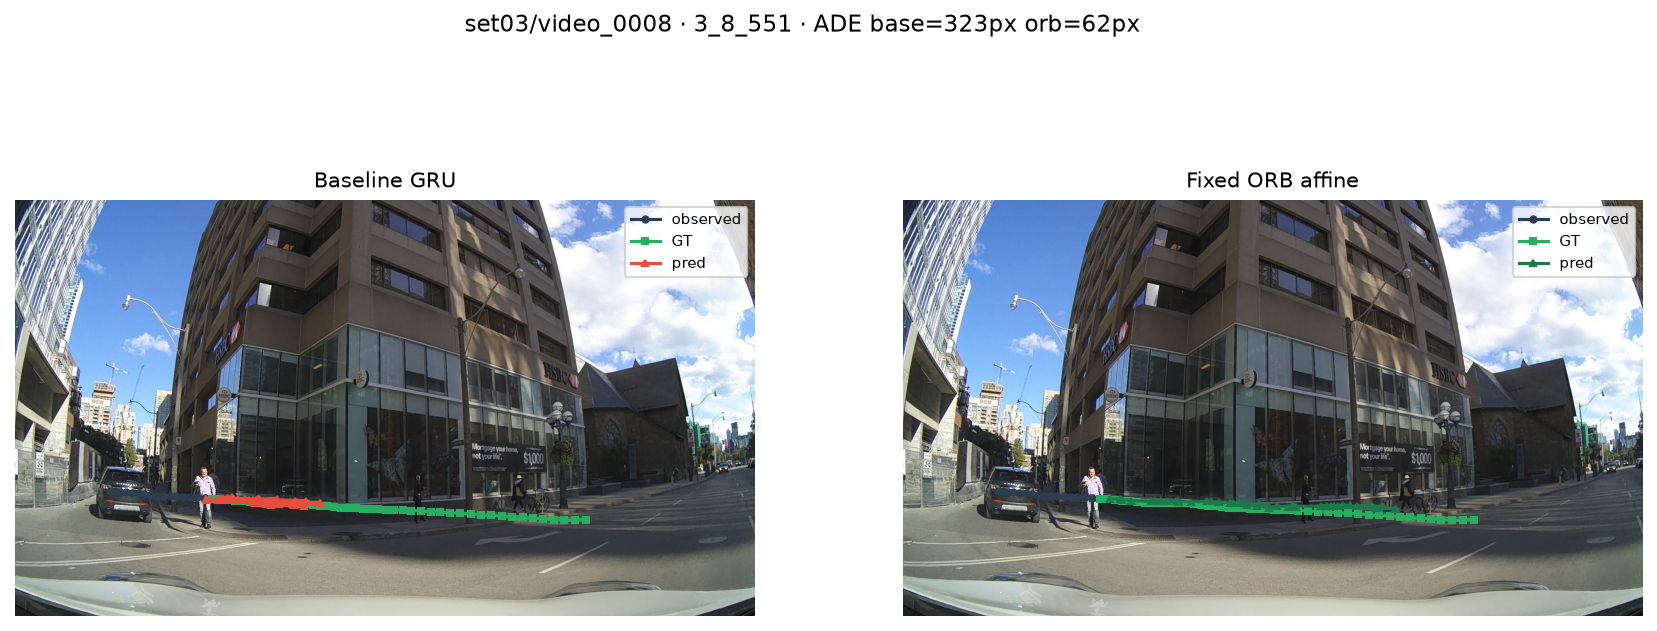
\includegraphics[width=\linewidth,height=0.16\textheight,keepaspectratio]{pie_compare_0.png}
    \caption{PIE trajectory overlay}
  \end{subfigure}\\[3pt]
  \begin{subfigure}[t]{0.48\linewidth}
    \centering
    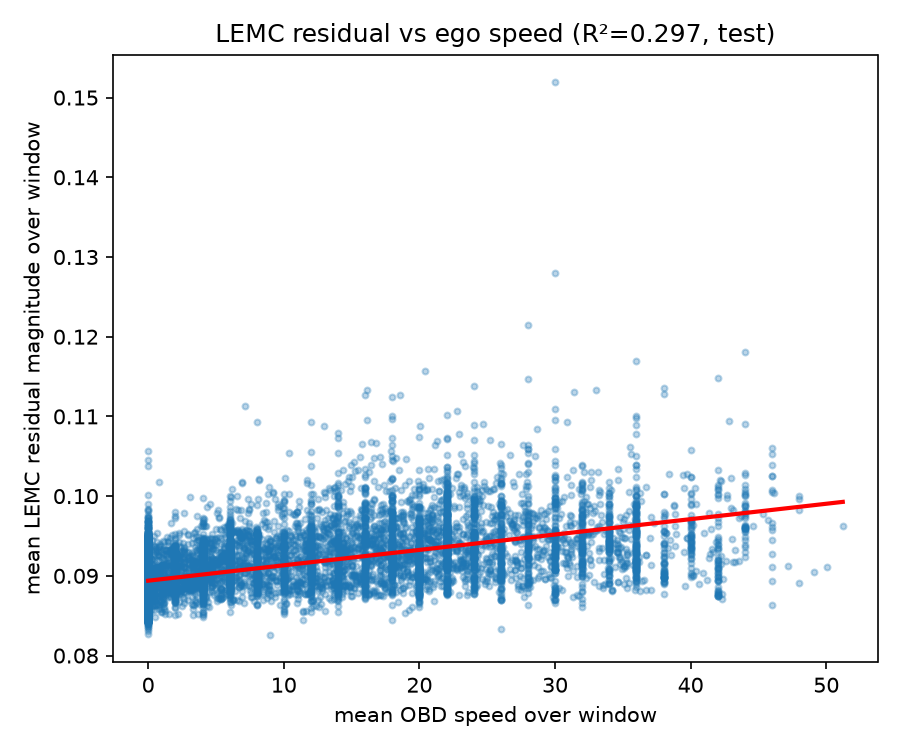
\includegraphics[width=\linewidth,height=0.16\textheight,keepaspectratio]{lemc_obd_scatter_pie_lemc_augmented_auxobd_seed0_test.png}
    \caption{LEMC vs.\ OBD ($R^2{=}0.30$)}
  \end{subfigure}\hfill
  \begin{subfigure}[t]{0.48\linewidth}
    \centering
    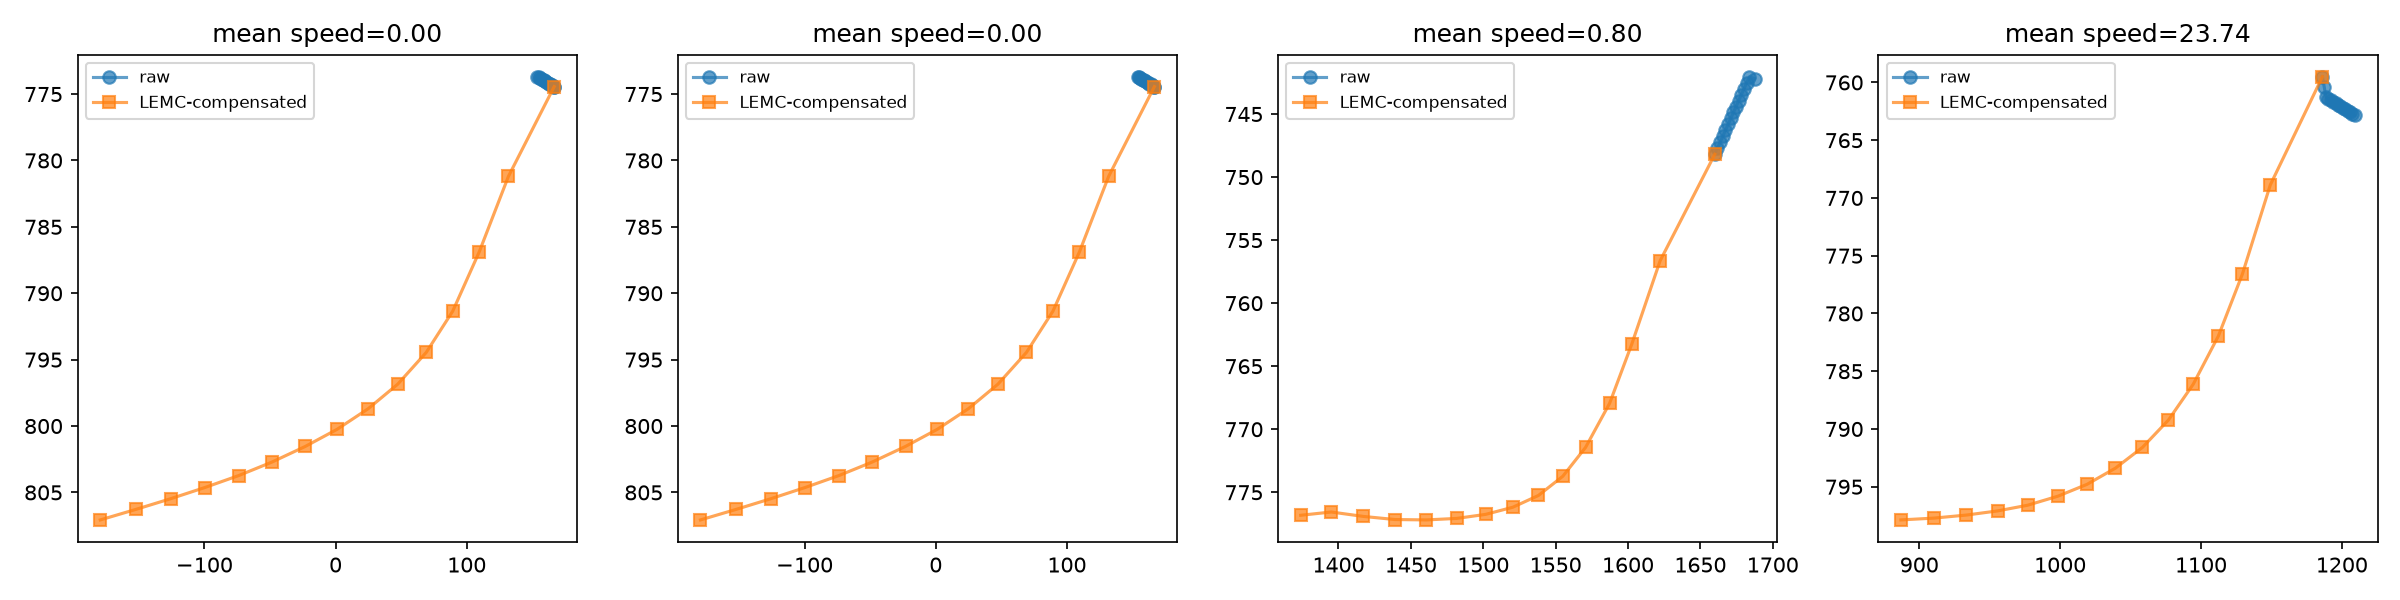
\includegraphics[width=\linewidth,height=0.16\textheight,keepaspectratio]{lemc_qualitative_pie_lemc_augmented_auxobd_seed0_test.png}
    \caption{LEMC failure (loops)}
  \end{subfigure}
  \caption{Qualitative results. (a) ORB flattens standing-pedestrian drift; (b) frame overlay; (c) LEMC correlates with speed but is physically invalid; (d) learned residual loops instead of compensating.}
  \label{fig:qual}
\end{figure}

\FloatBarrier

% ======================================================================
\section{Discussion}
\label{sec:discussion}

\textbf{Why does fixed geometry outperform learned residuals?}
A global 2-D shift cannot capture rotation and scale, whose apparent effect depends on image-plane position.
Multi-agent displacement statistics aggregate over pedestrians at different positions, so the learned residual fits a mean across inconsistent targets.
ORB-regression supervision does not resolve this: even when directly trained to predict ORB translations, LEMC fails the gate (33.4\%).
The failure mode is architectural, not data-limited.
This parallels Azarmi~\textit{et al.}'s~\cite{azarmi2024feature} finding that training-time correlation with a target is insufficient if the underlying physical process is not correctly represented.

\textbf{Why is PIE neutral while JAAD improves?}
On PIE, drivers typically reduce speed before pedestrians cross, creating a spurious statistical alignment between ego motion and pedestrian trajectory.
The uncompensated baseline already benefits from this alignment (the pedestrian is crossing while the car slows, reducing ego drift).
Fixed ORB removes this confound, leaving ADE essentially unchanged.
On JAAD, with no such OBD-mediated pre-alignment and higher vehicle speeds in some clips, raw tracks carry more uncompensated ego drift; removing it yields substantial ADE improvement.
This dissociation strengthens the causal argument: the gain is not due to compensation quality alone, but to the presence or absence of latent OBD alignment in the uncompensated tracks.

\textbf{Intent shortcut implications.}
The monotonic AUC ordering (0.80 $<$ 0.89 $<$ 0.93) across all PIE conditions suggests that intent AUC is partially inflated by ego-motion correlation rather than purely reflecting pedestrian intent.
Future intent benchmarks should either (a) evaluate after explicit ego-motion removal or (b) stratify by vehicle state to isolate pedestrian-specific variation.

\textbf{Limitations.}
Our backbone is a deliberately simple GRU on bbox coordinates.
ORB affine quality is degraded by depth variation (a scene-level depth confound caps $R^2$ at 0.41).
Missing affines (featureless frames) are imputed by holding the last valid affine.
JAAD intent AUC stays at chance because the dataset does not provide matched crossing labels per clip in our protocol.
Shortcut isolation relies on the variance gate rather than a dedicated causal intervention.

% ======================================================================
\section{Conclusion}
\label{sec:conclusion}

We showed that offline position-dependent ORB affine compensation passes a physical standing-pedestrian variance gate that three learned alternatives fail, while remaining trajectory-neutral on PIE ($-$0.5\% ADE) and improving JAAD by 25\% (20\,px absolute), with zero ego-motion sensors required at inference.
Intent AUC tracks available ego-motion (0.80 $\rightarrow$ 0.89 $\rightarrow$ 0.93): trajectory and intent benchmarks carry different information after compensation and should be reported separately.
The variance gate is a cheap, training-free filter that any proposed learned ego-motion module should pass before downstream evaluation; fixed offline geometry already does.
Configs, ORB extraction scripts, and three-seed checkpoints are released to support reproducible comparison on JAAD, a dataset that exposes ego-motion shortcuts invisible when OBD labels are always available.

\bibliographystyle{IEEEtran}
\bibliography{refs}

\end{document}
